\scanpage{116}
\[
H^*(\Delta^2T(A))\Longleftarrow(H^p\Delta^2)(H^q(K,A))
\]
\[
E_2^{pq}=\deleted{\unsure{H^p(\Delta^2H^qA)}}
\left\{\begin{array}{l}0\text{ si }q\neq0,\ p\unsure{\neq|=}q\\\phantom{0}\end{array}\right.
\]
\figure{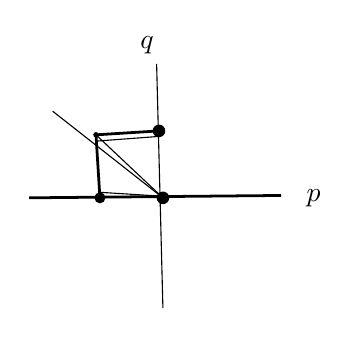
\begin{tikzpicture}
\draw[line width=1pt] (-1.7,0)--(1.5,.03);\node[right] at(1.7,0){$p$};
\draw (0,-1.4)--(-.08,1.7);\node[above] at(-.2,1.7){$q$};
\draw[line width=1pt] (-.8,0)--(-.85,.8)--(-.05,.85);
\draw (-1.4,1.1)--(0,0);\draw (-.85,.8)--(0,0);
\draw (-.85,.72)--(-.05,.78);\draw (-.8,.07)--(0,.02);
\fill (-.8,0) circle (.07);\fill(0,0) circle(.08);\fill(-.05,.85) circle(.08);\fill(-.85,.8) circle(.035);
\end{tikzpicture}}
\[
\left\{\begin{array}{l}
(H^{-1}\Delta^2)(H^0(K,A))\subset\pi_1(A)\\[1em]
(H^0\Delta^2)(H^0(K,A))\\[1em]
(H^0\Delta^2)(H^1(k,A))=H^1(k,A)
\end{array}\right.
\]
\margin{\uline{compact}}
\margin{\deleted{\unsure{qui est}}\inserted{\uline{est le \unsure{plus gr}}}
\uline{\unsure{complété}} de \uline{fini}}

$\Delta T(\mathcal P_\bullet)$ et $T(\mathcal P'_\bullet)$ \uuline{sont $=\unsure{0|\Delta}$.}
\[
\boxed{\underline{\underline{\operatorname{Ext}}}^{0}(\unsure{\mathcal P},\mathbb Q/\mathbb Z)=0}
\]
\[
\operatorname{Ext}(H
\]
\diagram{\begin{tikzcd}
T(\mathcal P')&\Delta T(\mathcal P_\bullet)\arrow[l,Leftarrow]
\end{tikzcd}}
\margin{\figure{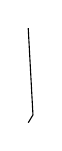
\begin{tikzpicture}\draw (0,1.2)--(.06,.1)--(0,0);\end{tikzpicture}}}

\deleted{\uline{Remarque} 2.7. J'ignore si les conditions
d'équidimensionnalité de 1.1. ii) sont
essentielles; de $=$ dans 2.6.

\uline{Prop.} 2.8. Continuité des Cohen-Macaulay.}
\mspage{115}

